\def\year{2016}\relax
%File: formatting-instruction.tex
\documentclass[letterpaper]{article}

\usepackage{aaai16}
\usepackage{graphicx}
\usepackage{times}
\usepackage{helvet}
%\usepackage{courier}
\frenchspacing
\setlength{\pdfpagewidth}{8.5in}
\setlength{\pdfpageheight}{11in}
\pdfinfo{
/Title (Bad News)
/Author (James Ryan, Ben Samuel, Adam Summerville, Michael Mateas, and Noah Wardrip-Fruin)
}
\setcounter{secnumdepth}{0}

\newcommand{\citealt}[1]{\citeauthor{#1} \shortcite{#1}}

\newcommand{\citealp}[1]{\citeauthor{#1}, \citeyear{#1}}


\begin{document}
% The file aaai.sty is the style file for AAAI Press 
% proceedings, working notes, and technical reports.

\title{\textit{Bad News}}

\author{James Ryan, Ben Samuel, Adam Summerville, Michael Mateas, and Noah Wardrip-Fruin \\
Expressive Intelligence Studio \\
University of California, Santa Cruz \\
\{jor, bsamuel, michaelm, nwf\}@soe.ucsc.edu, asummerv@ucsc.edu \\
@BadNewsGame
}

%James Ryan, Ben Samuel, Adam Summerville, \\
%\Large \textbf{Michael Mateas, and Noah Wardrip-Fruin} \\

%\author{AAAI Press\\
%Association for the Advancement of Artificial Intelligence\\
%2275 East Bayshore Road, Suite 160\\
%Palo Alto, California 94303\\
%}

\maketitle
\begin{abstract}
\textit{Bad News} is a novel playable experience that combines procedural generation, deep simulation, and live performance. Players explore procedurally generated American small towns inhabited by detailed characters with simulated backstories. Whenever the player encounters a resident, an improvisational actor reveals himself to perform the character live, adhering to his or her generated personality, life history, and subjective beliefs. With \textit{Bad News}, we strive to showcase the humor, drama, and tragedy of everyday life.
\end{abstract}


\section{How To Play}

It is the summer of 1979, and an unidentified resident of a small American town has died alone at home. The county mortician is responsible for identifying the body and notifying the next of kin, but a matter in a different part of the county demands his presence. Being occupied in this way, the mortician is forced to delegate this important task to his newly appointed assistant, the player. To carry out the task, the player must navigate the town and converse with its residents in order to obtain three crucial pieces of information, each of which can only be discovered by knowing the preceding piece: the identity of the deceased, given only the person's physical appearance and home; the identity of the next of kin, given the identity of the deceased and an explicit notion of a next of kin (that we provide); and the current location of the next of kin, given his or her identity and any other relevant information that the player has gathered. Finally, upon locating the next of kin, the player must notify him or her of the death. Throughout, she should remain discreet, so as to respect the privacy of the family.

The player sits on one side of a constructed model theatre (shown in Figure~\ref{fig:model_theatre}), with a tablet computer, a notebook, and a pen. A live actor sits across from the player, hidden by the theatre's adjustable curtain; behind a permanent lower curtain, a hidden screen displays a special actor interface and a discreet microphone captures sound. Out of sight, a \textit{wizard} listens to the audio feed. Gameplay always begins at the death scene, where the actor reveals himself to play the mortician, who explains what has happened and what the player must now do. This happens diegetically and occurs as embodied face-to-face conversation; the purpose of this scene is to subtly tutorialize and to gently ease the player into both the diegesis and the live-action role-playing that the experience requires. Crucially, the mortician and the player collaborate to construct a believable backstory that the player can rely on when talking with residents in the town---after all, it would not be discreet to openly parade as the mortician's assistant. From here, the mortician disappears by deploying the curtain, and the player is left with the tablet computer (see Figure~\ref{fig:player_interface}), which displays a player interface that initially describes her current location (including the body).

\begin{figure}[t]
  \centering
  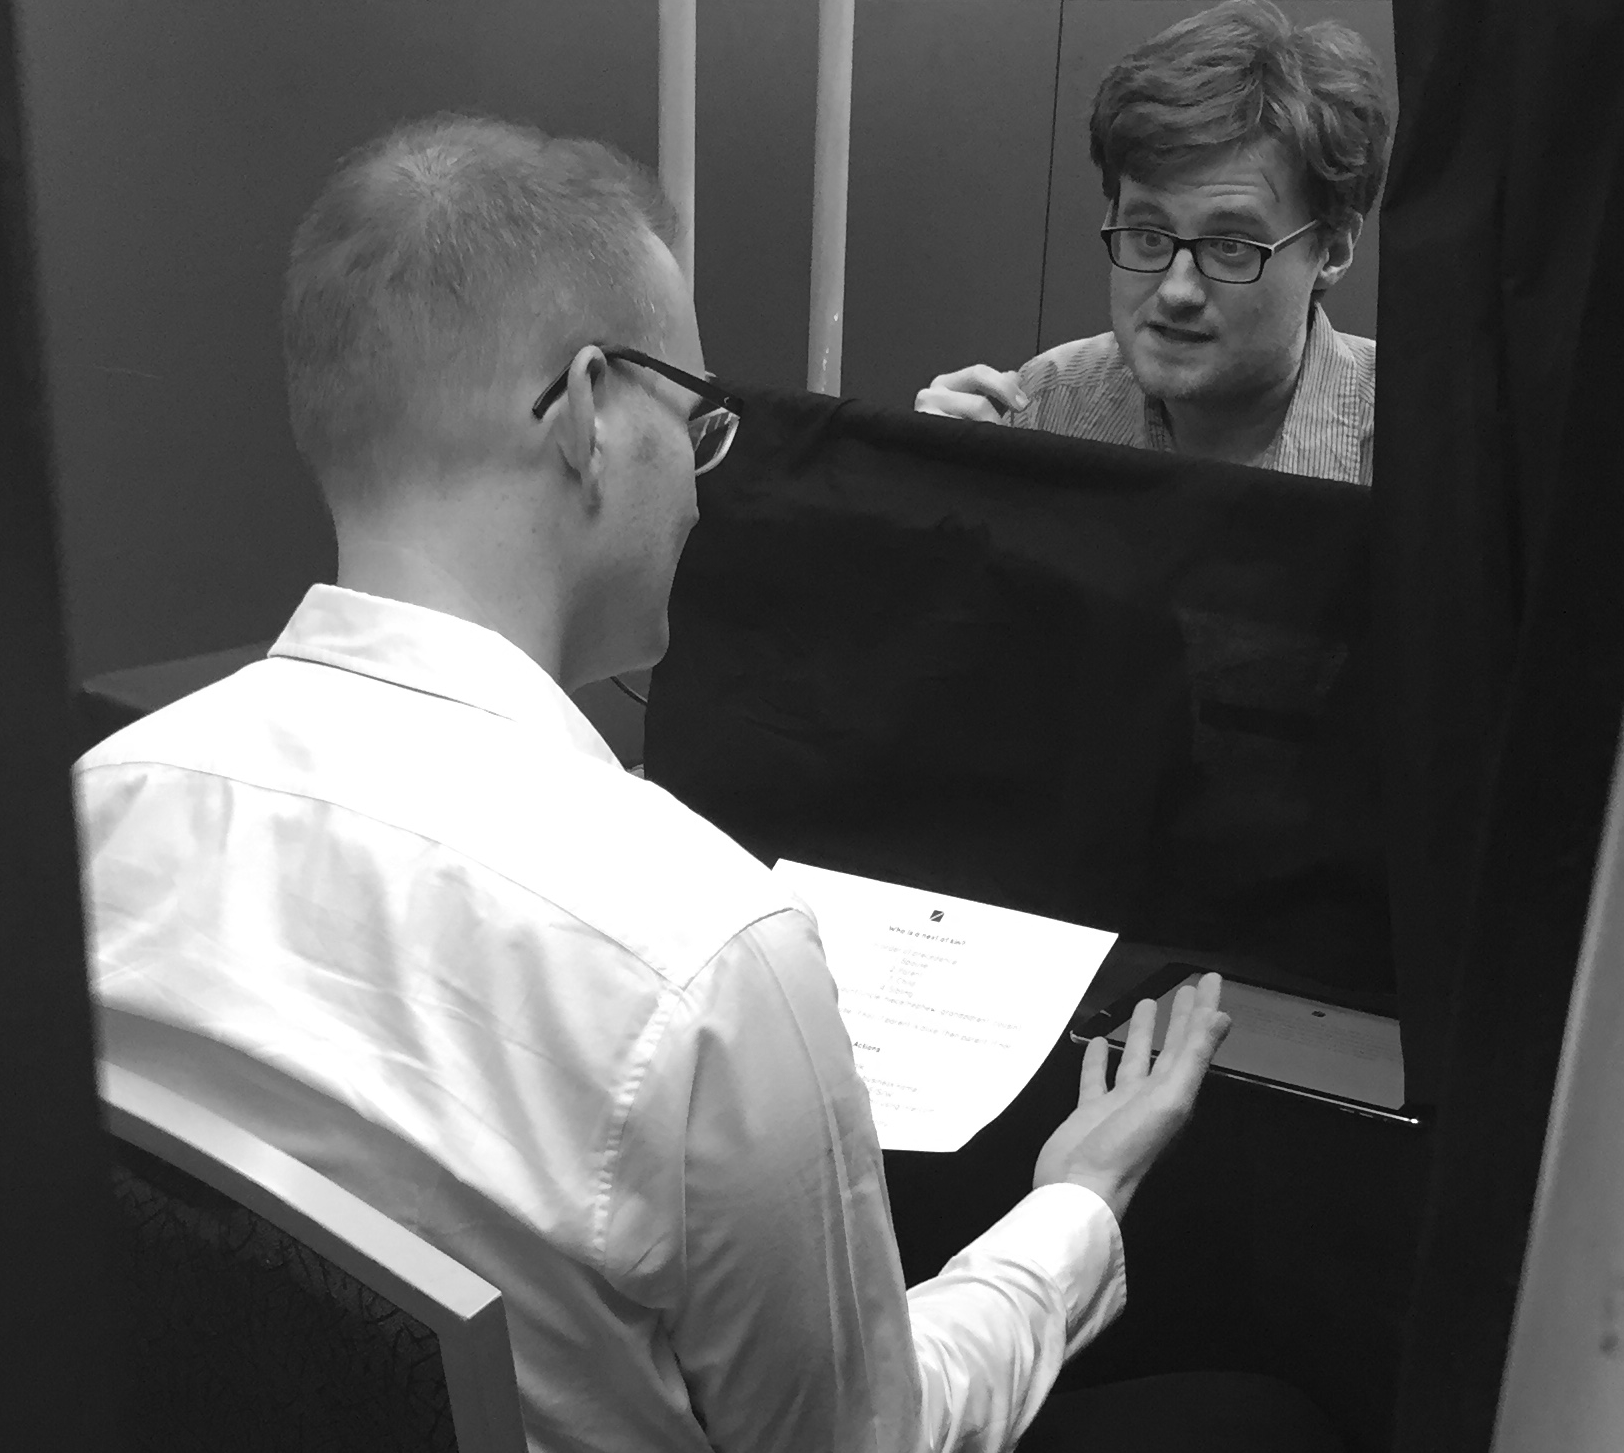
\includegraphics[width=0.8\columnwidth]{player_and_actor.png}
%  \vspace{-2.0em}
  \caption{A player, left, engages in embodied conversation with the actor, who improvisationally performs as a resident of the town.}
  \label{fig:player_and_actor}
\end{figure}

From here, the player proceeds by speaking commands aloud; the wizard executes these throughout the experience by live-coding modifications to the simulation in real time. Permissible commands include moving about the town (in a direction, or to an address), viewing a residential or business directory, approaching a character to engage in conversation, and more. As the player moves about the town, her interface updates to describe her current location. When a player approaches a town resident, the hidden actor interface updates to display details about that character's personality, life history, and subjective beliefs. After spending a few moments preparing for the role, the actor pulls back the curtain to play that character live. As the subject of conversation shifts between residents of the town, the wizard crucially updates the actor interface to display the character's beliefs about that particular resident. Meanwhile, the wizard queries the simulation for narrative intrigue (again by live-coding), which he can deliver to the actor directly through a live chat session (\textit{e.g.}, ``you went to high school with the subject''). Gameplay ends once the player notifies the next of kin of the death. A typical session lasts roughly 45 minutes, though the wizard and actor can coordinate in real time to control this. For more details, see our longer paper \cite{samuel2016bad}.


\section{Why To Play}


\begin{figure}[t]
  \centering
  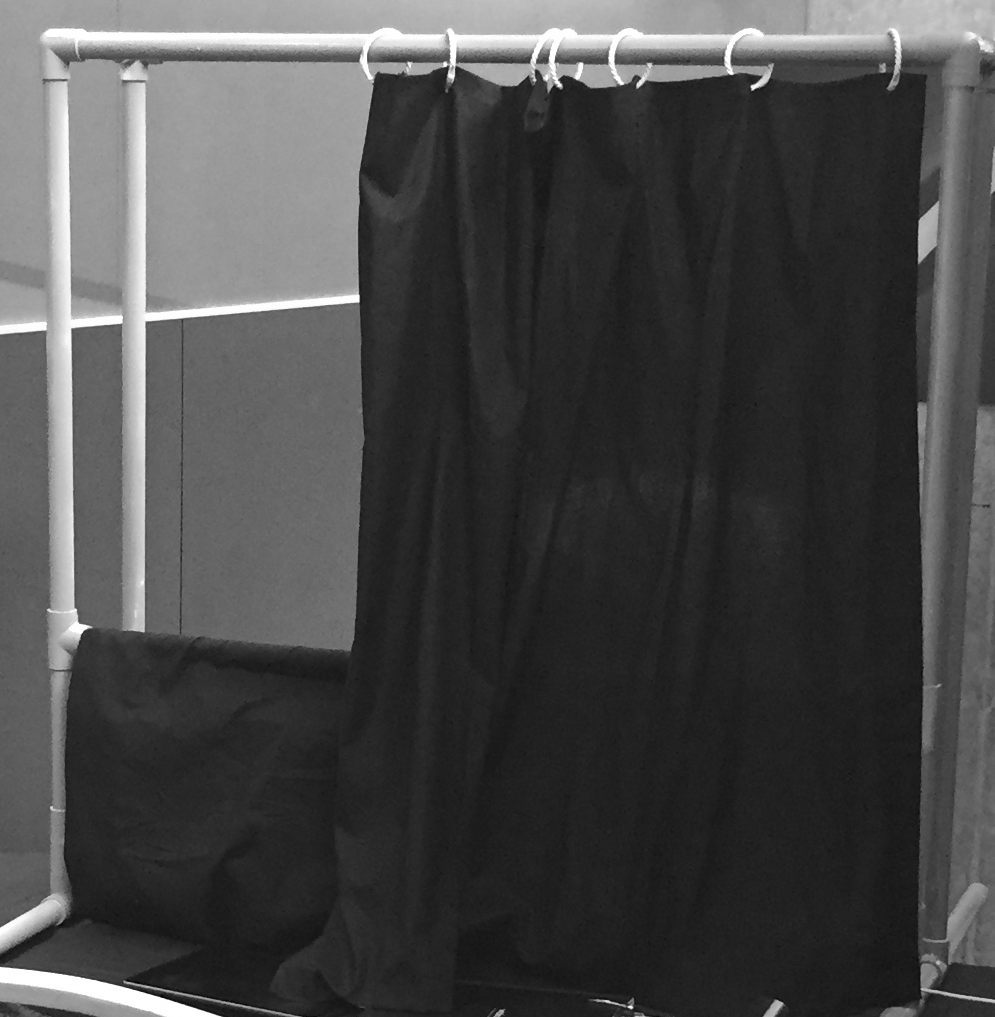
\includegraphics[width=0.64\columnwidth]{the_puppet_theatre.png}
%  \vspace{-2.0em}
  \caption{A constructed model theatre separates the player and our live actor.}
  \label{fig:model_theatre}
\end{figure}

\textit{Bad News} is appealing as a novel, AI-driven, and tender experience. While \textit{mixed reality} is a growing and fairly active area \cite{ohta2014mixed}, there are surprisingly few media works that specifically combine computation and live improvisation. In fact, we are aware of only two other examples of this---\textit{Coffee: A Misunderstanding} \cite{squinkifer2014coffee} and \textit{S\'{e}ance} \cite{seance}---though interest is growing \cite{martens2016towards}. Incidentally, \textit{S\'{e}ance} features our same actor, Ben Samuel, who appears to be the world's expert in improvisational acting under computational constraints; watching him perform in myriad roles is a core appeal of the experience. Beyond its novelty, this work is deeply AI-driven. Each \textit{Bad News} town is procedurally generated using the \textit{Talk of the Town} AI framework \cite{ryan2015toward}. Specifically, towns are simulated for 140 years of diegetic time, yielding hundreds of residents who are socially embedded and who harbor subjective beliefs about the town (which may be wrong for multiple interesting reasons). This provides an abundance of narrative material and dramatic intrigue (\textit{e.g.}, family feuds, love triangles, struggling businesses) that exceeds the capacities of a 45-minute playthrough and that could not have tractably been hand-authored. Several players have reported feeling like they were \textit{transported} to the generated towns that they visited \cite{green2004understanding}. Finally, \textit{Bad News} is a tender experience. As a game about death notification, it compels the player to be sincere and tactful---many have commented on the emotional intensity of their notification scenes. Set in run-of-the-mill American small towns, we strive in each playthrough, through acting and wizardry, to showcase the humor, drama, and tragedy of everyday life.

\vspace{-0.4em}
\section{Where To Play}

\begin{figure}[t]
  \centering
  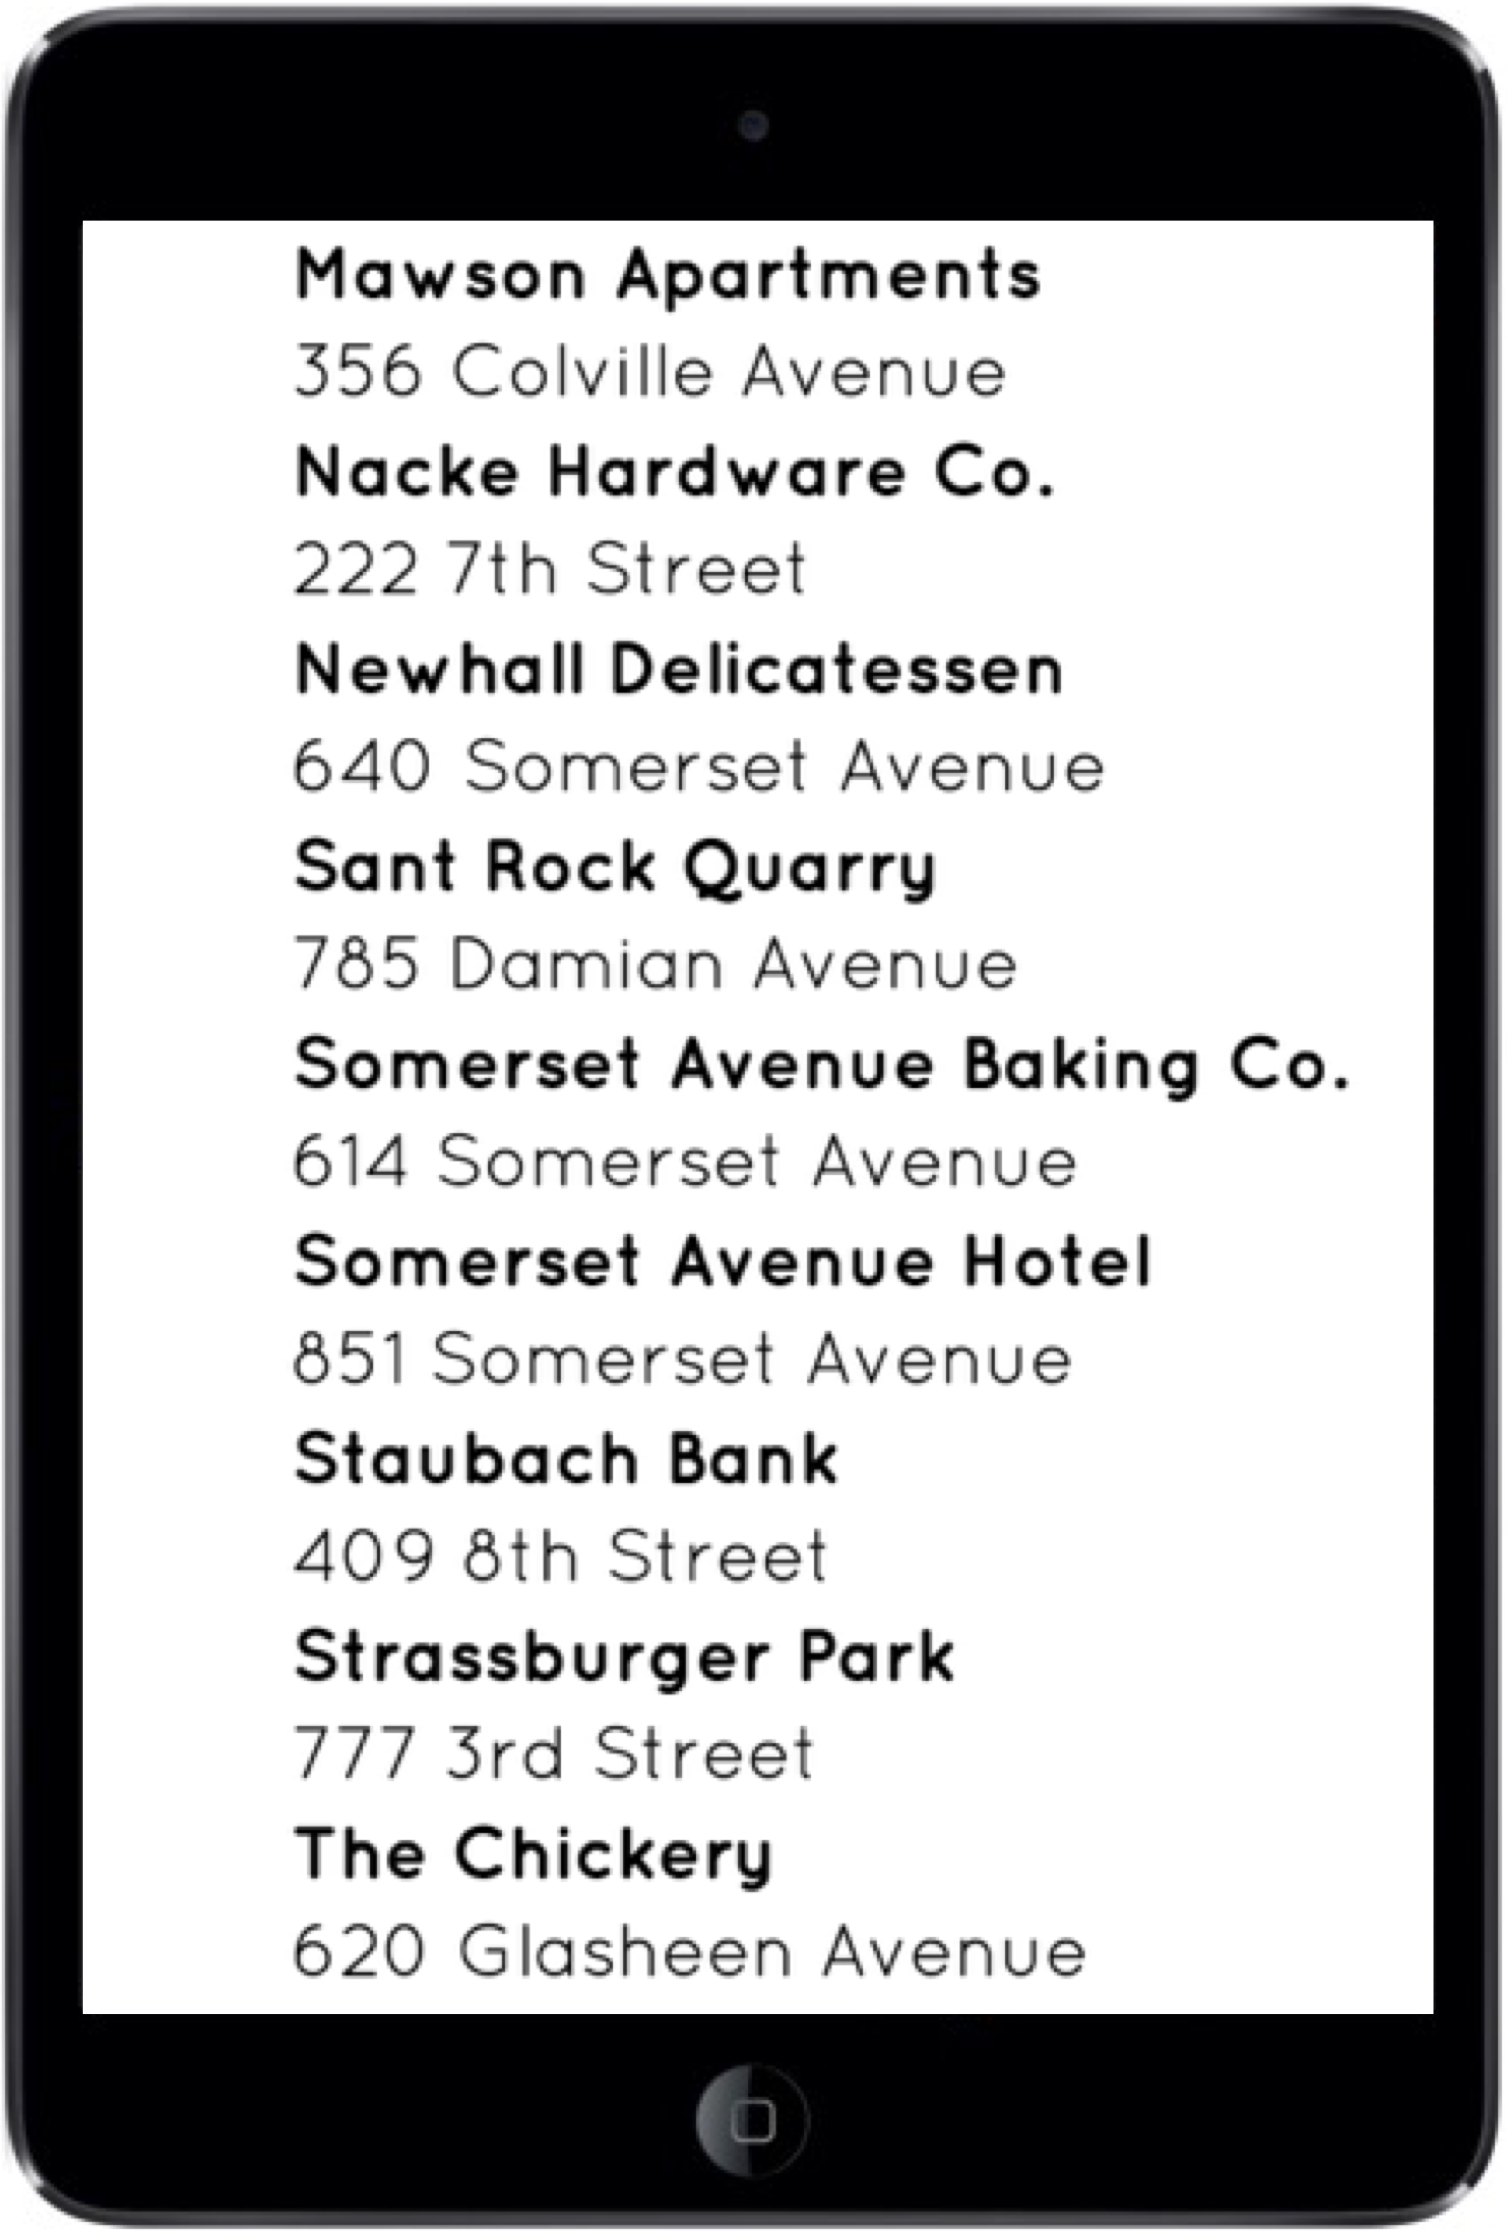
\includegraphics[width=0.42\columnwidth]{player_interface.png}
%  \vspace{-2.0em}
  \caption{Excerpt from a business directory for a procedurally generated town, as displayed on the player interface.}
  \label{fig:player_interface}
\end{figure}

Because the actor and wizard must both be present, \textit{Bad News} can only be played in person at scheduled performances. Though we have accommodated private requests, it is primarily intended as an exhibition piece. An early test incarnation was conducted at the 2015 Experimental AI in Games workshop in Santa Cruz \cite{ryan2015bad}, and more recently our refined, longer version was performed at the ACM Conference on Human Factors in Computing Systems (CHI) in San Jose \cite{ryan2016bad} and at Gamenest in San Francisco. The middle performance was part of the Innovative Game Design track of the CHI Student Game Competition, which \textit{Bad News} won.

\vspace{-0.4em}
\bibliographystyle{aaai}
\bibliography{bad_news_AIIDE_PE}

\end{document}


%\begin{quote}
%\begin{small}
%\textbackslash documentclass[letterpaper]{article}\\
%\% \textit{Required Packages}\\
%\textbackslash usepackage\{aaai\}\\
%\textbackslash usepackage\{times\}\\
%\textbackslash usepackage\{helvet\}\\
%\textbackslash usepackage\{courier\}\\
%\textbackslash setlength\{\textbackslash pdfpagewidth\}\{8.5in\}
%\textbackslash setlength\{\textbackslash pdfpageheight\}\{11in\}\\
%\%\%\%\%\%\%\%\%\%\%\\
%\% \textit{PDFINFO for PDF\LaTeX{}}\\
%\% Uncomment and complete the following for metadata (your paper must compile with PDF\LaTeX{})\\
%\textbackslash pdfinfo\{\\
%/Title (Input Your Paper Title Here)\\
%/Author (John Doe, Jane Doe)\\
%/Keywords (Input your paper's keywords in this optional area)\\
%\}\\
%\%\%\%\%\%\%\%\%\%\%\\
%\% \textit{Section Numbers}\\
%\% Uncomment if you want to use section numbers\\
%\% and change the 0 to a 1 or 2\\
%\% \textbackslash setcounter\{secnumdepth\}\{0\}\\
%\%\%\%\%\%\%\%\%\%\%\\
%\% \textit{Title, Author, and Address Information}\\
%\textbackslash title\{Title\}\\
%\textbackslash author\{Author 1 \textbackslash and Author 2\textbackslash\textbackslash \\ 
%Address line\textbackslash\textbackslash\\ Address line\textbackslash\textbackslash \\
%\textbackslash And\\
%Author 3\textbackslash\textbackslash\\ Address line\textbackslash\textbackslash\\ Address line\}\\
%\%\%\%\%\%\%\%\%\%\%\\
%\% \textit{Body of Paper Begins}\\
%\textbackslash begin\{document\}\\
%\textbackslash maketitle\\
%...\\
%\%\%\%\%\%\%\%\%\%\%\\
%\% \textit{References and End of Paper}\\
%\textbackslash bibliography\{Bibliography-File\}\\
%\textbackslash bibliographystyle\{aaai\}\\
%\textbackslash end\{document\}
%\end{small}
%\end{quote}
%
%The following packages are incompatible with aaai.sty and/or aaai.bst and must not be used (this list is not exhaustive --- there are others as well):
%\begin{itemize}
%\item authblk
%\item fullpage
%\item hyperref
%\item natbib
%\item geometry
%\item titlesec
%\item layout
%\item caption
%\item titlesec
%\item savetrees
%\item T1 fontenc package (install the CM super fonts package instead)
%\end{itemize}